\documentclass[11pt]{article}
\usepackage{tikz}
\usetikzlibrary{automata}
\usetikzlibrary{shapes.geometric}
\usetikzlibrary{calc}
\usetikzlibrary{decorations.pathmorphing}
\usetikzlibrary{decorations.markings}
\usepackage{amsmath,amsfonts,latexsym,amscd,amssymb,theorem}
\usepackage[ansinew]{inputenc}
\usepackage{amsmath}
\usepackage{amssymb}

\begin{document}

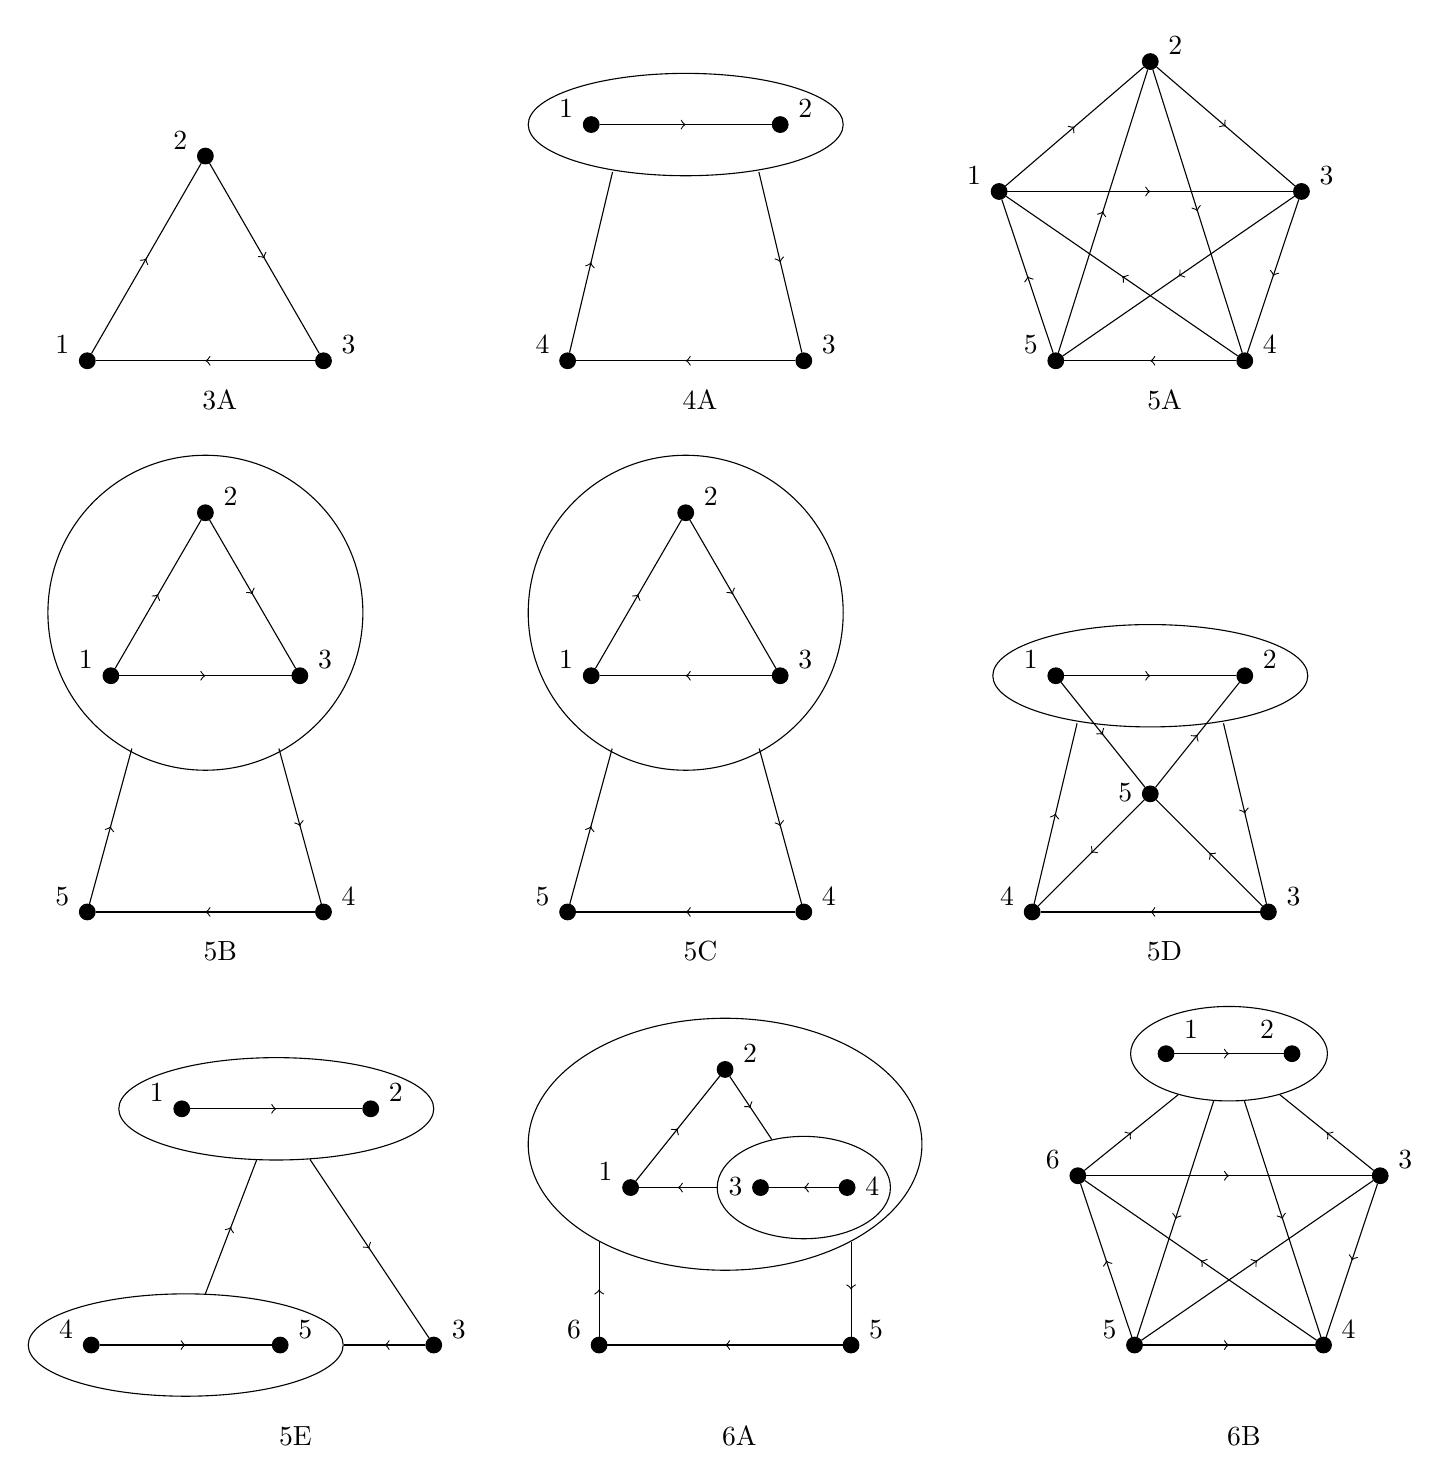
\begin{tikzpicture}
\tikzset{enclosed/.style={draw,circle,inner sep=2pt,minimum size=4pt,fill=black}}
\tikzset{->-/.style={decoration={
            markings,
            mark=at position #1 with
            {\arrow{>}}},postaction={decorate}}}
\node[enclosed,label={left,yshift=.2cm:1}](1)at(0,0){};
\node[enclosed,label={left,yshift=.2cm:2}](2)at(1.5,2.6){};
\node[enclosed,label={right,yshift=.2cm:3}](3)at(3,0){};
\draw[black,->-=.5] (1)--(2);
\draw[black,->-=.5] (2)--(3);
\draw[black,->-=.5] (3)--(1);

\node[minimum size=.1pt,label={left:3A}](3A)at(2.15,-.5){};



\node[ellipse,minimum width=4cm,minimum height=1.3cm,draw](4Aa)at(7.6,3){};
\node[minimum size=.1pt](4Aa1)at(6.7,2.52){};
\node[minimum size=.1pt](4Aa2)at(8.5,2.52){};
\node[enclosed,label={left,yshift=.2cm:1}](4A1)at(6.4,3){};
\node[enclosed,label={right,yshift=.2cm:2}](4A2)at(8.8,3){};
\draw[black,->-=.5] (4A1)--(4A2);
\node[enclosed,label={right,yshift=.2cm:3}](4A3)at(9.1,0){};
\node[enclosed,label={left,yshift=.2cm:4}](4A4)at(6.1,0){};
\draw[black,->-=.5] (4A3)--(4A4);
\draw[black,->-=.5] (4A4)--(4Aa1);
\draw[black,->-=.5] (4Aa2)--(4A3);

\node[minimum size=.1pt,label={left:4A}](4A)at(8.25,-.5){};





\node[enclosed,label={left,yshift=.2cm:1}](5A1)at(11.58,2.15){};
\node[enclosed,label={right,yshift=.2cm:2}](5A2)at(13.5,3.8){};
\node[enclosed,label={right,yshift=.2cm:3}](5A3)at(15.42,2.15){};
\node[enclosed,label={right,yshift=.2cm:4}](5A4)at(14.7,0){};\node[enclosed,label={left,yshift=.2cm:5}](5A5)at(12.3,0){};

\draw[black,->-=.5] (5A1)--(5A2);
\draw[black,->-=.5] (5A1)--(5A3);
\draw[black,->-=.5] (5A2)--(5A3);
\draw[black,->-=.5] (5A2)--(5A4);
\draw[black,->-=.5] (5A3)--(5A4);
\draw[black,->-=.5] (5A3)--(5A5);
\draw[black,->-=.5] (5A4)--(5A5);
\draw[black,->-=.5] (5A4)--(5A1);
\draw[black,->-=.5] (5A5)--(5A1);
\draw[black,->-=.5] (5A5)--(5A2);

\node[minimum size=.1pt,label={left:5A}](5A)at(14.15,-.5){};








\node[ellipse,minimum width=4cm,minimum height=4cm,draw](5Ba)at(1.5,-3.2){};
\node[minimum size=.1pt](5Ba1)at(0.6,-4.8){};
\node[minimum size=.1pt](5Ba2)at(2.4,-4.8){};
\node[enclosed,label={left,yshift=.2cm:1}](5B1)at(0.3,-4){};
\node[enclosed,label={right,yshift=.2cm:2}](5B2)at(1.5,-1.93){};\node[enclosed,label={right,yshift=.2cm:3}](5B3)at(2.7,-4){};
\draw[black,->-=.5] (5B1)--(5B2);
\draw[black,->-=.5] (5B2)--(5B3);
\draw[black,->-=.5] (5B1)--(5B3);
\node[enclosed,label={right,yshift=.2cm:4}](5B4)at(3,-7){};
\node[enclosed,label={left,yshift=.2cm:5}](5B5)at(0,-7){};
\draw[black,->-=.5] (5B4)--(5B5);
\draw[black,->-=.5] (5B5)--(5Ba1);
\draw[black,->-=.5] (5Ba2)--(5B4);

\node[minimum size=.1pt,label={left:5B}](5B)at(2.15,-7.5){};










\node[ellipse,minimum width=4cm,minimum height=4cm,draw](5Ca)at(7.6,-3.2){};
\node[minimum size=.1pt](5Ca1)at(6.7,-4.8){};
\node[minimum size=.1pt](5Ca2)at(8.5,-4.8){};
\node[enclosed,label={left,yshift=.2cm:1}](5C1)at(6.4,-4){};
\node[enclosed,label={right,yshift=.2cm:2}](5C2)at(7.6,-1.93){};\node[enclosed,label={right,yshift=.2cm:3}](5C3)at(8.8,-4){};
\draw[black,->-=.5] (5C1)--(5C2);
\draw[black,->-=.5] (5C2)--(5C3);
\draw[black,->-=.5] (5C3)--(5C1);
\node[enclosed,label={right,yshift=.2cm:4}](5C4)at(9.1,-7){};
\node[enclosed,label={left,yshift=.2cm:5}](5C5)at(6.1,-7){};
\draw[black,->-=.5] (5C4)--(5C5);
\draw[black,->-=.5] (5C5)--(5Ca1);
\draw[black,->-=.5] (5Ca2)--(5C4);

\node[minimum size=.1pt,label={left:5C}](5C)at(8.25,-7.5){};










\node[ellipse,minimum width=4cm,minimum height=1.3cm,draw](5D)at(13.5,-4){};
\node[minimum size=.1pt](5Da1)at(12.6,-4.48){};
\node[minimum size=.1pt](5Da2)at(14.4,-4.48){};
\node[enclosed,label={left,yshift=.2cm:1}](5D1)at(12.3,-4){};
\node[enclosed,label={right,yshift=.2cm:2}](5D2)at(14.7,-4){};
\draw[black,->-=.5] (5D1)--(5D2);
\node[enclosed,label={right,yshift=.2cm:3}](5D3)at(15,-7){};
\node[enclosed,label={left,yshift=.2cm:4}](5D4)at(12,-7){};
\draw[black,->-=.5] (5D3)--(5D4);
\draw[black,->-=.5] (5D4)--(5Da1);
\draw[black,->-=.5] (5Da2)--(5D3);
\node[enclosed,label={left,yshift=.01cm:5}](5D5)at(13.5,-5.5){};
\draw[black,->-=.5] (5D1)--(5D5);
\draw[black,->-=.5] (5D3)--(5D5);
\draw[black,->-=.5] (5D5)--(5D2);
\draw[black,->-=.5] (5D5)--(5D4);

\node[minimum size=.1pt,label={left:5D}](5D)at(14.15,-7.5){};














\node[ellipse,minimum width=4cm,minimum height=1.3cm,draw](5Ea)at(2.4,-9.5){};
\node[minimum size=.1pt](5Ea1)at(1.5,-9.98){};
\node[minimum size=.1pt](5Ea2)at(3.3,-9.98){};
\node[enclosed,label={left,yshift=.2cm:1}](5E1)at(1.2,-9.5){};
\node[enclosed,label={right,yshift=.2cm:2}](5E2)at(3.6,-9.5){};
\draw[black,->-=.5] (5E1)--(5E2);
\node[enclosed,label={right,yshift=.2cm:3}](5E3)at(4.4,-12.5){};
\node[ellipse,minimum width=4cm,minimum height=1.3cm,draw](5Eb)at(1.25,-12.5){};
\node[enclosed,label={left,yshift=.2cm:4}](5E4)at(0.05,-12.5){};
\node[enclosed,label={right,yshift=.2cm:5}](5E5)at(2.45,-12.5){};
\draw[black,->-=.5] (5E3)--(5Eb);
\draw[black,->-=.5] (5Ea)--(5E3);
\draw[black,->-=.5] (5E4)--(5E5);
\draw[black,->-=.5] (5Eb)--(5Ea);

\node[minimum size=.1pt,label={left:5E}](5E)at(3.1,-13.65){};













\node[ellipse,minimum width=5cm,minimum height=3.2cm,draw](6Aa)at(8.1,-9.95){};
\node[minimum size=.1pt](6Aa1)at(6.5,-11.07){};
\node[minimum size=.1pt](6Aa2)at(9.7,-11.07){};
\node[ellipse,minimum width=2.2cm,minimum height=1.3cm,draw](6Ab)at(9.1,-10.5){};
\node[enclosed,label={left,yshift=.2cm:1}](6A1)at(6.9,-10.5){};
\node[enclosed,label={right,yshift=.2cm:2}](6A2)at(8.1,-9){};
\node[enclosed,label={left,yshift=.01cm:3}](6A3)at(8.55,-10.5){};
\node[enclosed,label={right,yshift=.01cm:4}](6A4)at(9.65,-10.5){};\node[enclosed,label={right,yshift=.2cm:5}](6A5)at(9.7,-12.5){};\node[enclosed,label={left,yshift=.2cm:6}](6A6)at(6.5,-12.5){};

\draw[black,->-=.5] (6A1)--(6A2);
\draw[black,->-=.5] (6A2)--(6Ab);
\draw[black,->-=.5] (6Ab)--(6A1);
\draw[black,->-=.5] (6A4)--(6A3);
\draw[black,->-=.5] (6Aa2)--(6A5);
\draw[black,->-=.5] (6A5)--(6A6);
\draw[black,->-=.5] (6A6)--(6Aa1);

\node[minimum size=.1pt,label={left:6A}](6A)at(8.75,-13.65){};









\node[enclosed,label={left,yshift=.2cm:6}](6B6)at(12.58,-10.35){};

\node[ellipse,minimum width=2.5cm,minimum height=1.2cm,draw](6Ba)at(14.5,-8.8){};

\node[enclosed,label={right,yshift=.3cm:1}](6B1)at(13.7,-8.8){};
\node[enclosed,label={left,yshift=.3cm:2}](6B2)at(15.3,-8.8){};
\node[enclosed,label={right,yshift=.2cm:3}](6B3)at(16.42,-10.35){};
\node[enclosed,label={right,yshift=.2cm:4}](6B4)at(15.7,-12.5){};\node[enclosed,label={left,yshift=.2cm:5}](6B5)at(13.3,-12.5){};
\draw[black,->-=.5] (6B1)--(6B2);
\draw[black,->-=.5] (6B6)--(6Ba);
\draw[black,->-=.5] (6B6)--(6B3);
\draw[black,->-=.5] (6Ba)--(6B5);
\draw[black,->-=.5] (6Ba)--(6B4);
\draw[black,->-=.5] (6B3)--(6B4);
\draw[black,->-=.5] (6B3)--(6Ba);
\draw[black,->-=.5] (6B5)--(6B4);
\draw[black,->-=.5] (6B4)--(6B6);
\draw[black,->-=.5] (6B5)--(6B6);
\draw[black,->-=.5] (6B5)--(6B3);

\node[minimum size=.1pt,label={left:6B}](6B)at(15.15,-13.65){};

\end{tikzpicture}

\end{document}